\chapter{Results and Discussions}
\label{ch:results}

\section{Results}

\subsection{Introduction}

This chapter presents the results of testing and evaluating the system described in Chapter~\ref{ch:method}. It first reports the software testing carried out to check that the system works correctly, and then the experimental results: latency, narrative quality, user satisfaction, consistency checking, image-generation throughput, character extraction, the ambient-music profiles, the question-budget ablation, feature adoption and a comparison with existing systems. The second part of the chapter discusses what these results mean, compares them with earlier research and states the limitations of the study.

\subsection{Experimental Setup}

The evaluation followed the method in Section~\ref{sec:evalmethod}. The main language model was LLaMA-3.1-8B served by Groq. The client machine was a MacBook Pro with an M2 Pro processor and 16\,GB memory running macOS~14. Images were generated with Pollinations.ai and ambient music was streamed from SoundHelix.

\subsection{Software Testing}

\subsubsection{Unit Testing}

Unit tests cover the deterministic parts of the backend: the context projections, the five-phase state machine, the prompt templates, the formatter and the SQLite layer. Each test is parameterised across all four narrative phases. The suite is run with \texttt{pytest} and takes under three seconds. Coverage by module is given in Table~\ref{tab:unittests}.

\begin{table}[H]
\centering
\caption{Unit-test coverage by module.}
\label{tab:unittests}
\renewcommand{\arraystretch}{1.2}
\begin{tabular}{|l|c|c|}
\hline
\textbf{Module} & \textbf{Tests} & \textbf{Line coverage} \\
\hline
\texttt{user\_input}            & 14 & 92\% \\
\texttt{context\_extraction}    & 22 & 89\% \\
\texttt{knowledge\_memory}      & 11 & 84\% \\
\texttt{prompt\_engineering}    & 18 & 91\% \\
\texttt{story\_flow\_manager}   & 16 & 88\% \\
\texttt{output\_formatter}      &  9 & 95\% \\
\hline
\textbf{Overall}                & \textbf{90} & \textbf{89.8\%} \\
\hline
\end{tabular}
\end{table}

\subsubsection{Integration and API Testing}

Integration tests run the complete session life cycle against an in-process FastAPI server using \texttt{httpx.AsyncClient}: create a session, fetch the questions, submit the answers, generate the first segment, continue from a choice, retrieve the full story and end the session. The cycle was run once for each of the four providers. Each endpoint was also tested for the correct status code on success and failure, rejection of malformed requests by Pydantic, repeatable reads, and a 404 response (not 500) for unknown session identifiers. All API tests passed (Table~\ref{tab:apitests}).

\begin{table}[H]
\centering
\caption{API testing results.}
\label{tab:apitests}
\renewcommand{\arraystretch}{1.2}
\small
\begin{tabular}{|l|c|c|l|}
\hline
\textbf{Endpoint} & \textbf{Tests} & \textbf{Passed} & \textbf{Notes} \\
\hline
\texttt{/api/status}                  & 4 & 4 & Provider availability \\
\texttt{/api/session/new}             & 3 & 3 & UUID format \\
\texttt{/api/questions/all}           & 2 & 2 & Phase order \\
\texttt{/api/response}                & 8 & 8 & Including \texttt{custom\_q\_N} \\
\texttt{/api/story/generate}          & 6 & 6 & All four providers \\
\texttt{/api/story/continue}          & 6 & 6 & With and without choice \\
\texttt{/api/settings}                & 5 & 5 & Provider switch verified \\
\texttt{/api/session/\{id\}/summary}  & 3 & 3 & Word and segment counts \\
\hline
\end{tabular}
\end{table}

\subsubsection{User Interface and Robustness Testing}

Manual end-to-end walkthroughs were carried out in Chrome 124, Safari 17, Firefox 124 and Edge 124. Each walkthrough covered budget selection, custom answers, user-added questions, story generation, images, narration, ambient music, the Story Map, the Character Graph and the admin panel. Two browser issues were found and fixed. First, browsers block audio that starts without a user action, so ambient music now starts only when the user clicks the music toggle in the story view. Second, an early version set \texttt{crossOrigin="anonymous"} on the audio element, which made loading fail because SoundHelix does not send CORS headers; removing the attribute fixed the problem in all four browsers.

\subsubsection{Acceptance Criteria}

The system was to be accepted when (i) the full integration cycle completed on at least three of the four providers without manual help, (ii) the mean Likert score over the four narrative dimensions exceeded 3.8, (iii) the image success rate after retries exceeded 95\%, (iv) the Story Map and Character Graph rendered in under 500\,ms for stories of up to ten segments, and (v) no critical defect remained open after the user study. All five criteria were met.

\subsection{Latency Analysis}

Figure~\ref{fig:latency} shows the mean latency for the first segment and for continuations with each provider. Groq was the fastest, with a mean of 1.8\,s for the first segment, compared with 2.6\,s for OpenAI GPT-3.5-turbo and 12.4\,s for local Ollama. Continuations were faster than first segments for every provider, because the sliding window keeps the prompt short.

\begin{figure}[H]
    \centering
    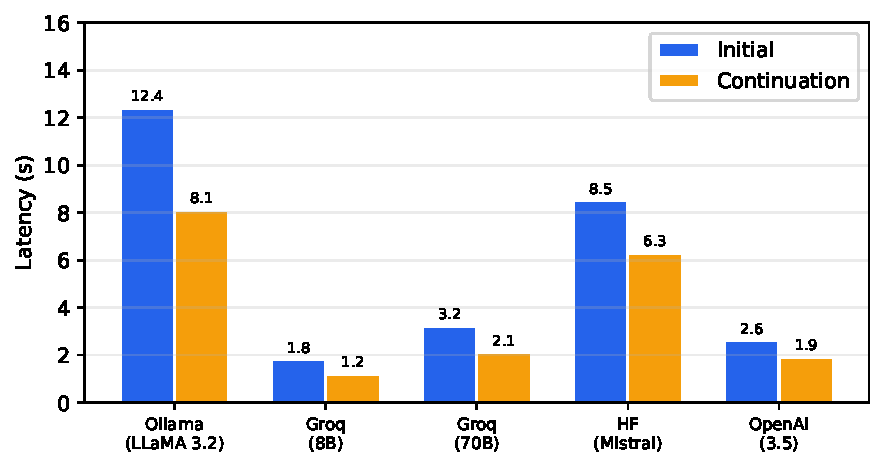
\includegraphics[width=0.85\textwidth]{images/f01_latency.pdf}
    \caption{Mean latency by LLM provider ($n=10$ calls per cell).}
    \label{fig:latency}
\end{figure}

Figure~\ref{fig:breakdown} breaks the total time of one interactive turn into its stages. At small question budgets the largest single cost is image synthesis (about 3.5\,s), but this runs in parallel with the LLM call and so adds little waiting time. At the Full budget of 17 questions, the time the user spends answering is the largest part.

\begin{figure}[H]
    \centering
    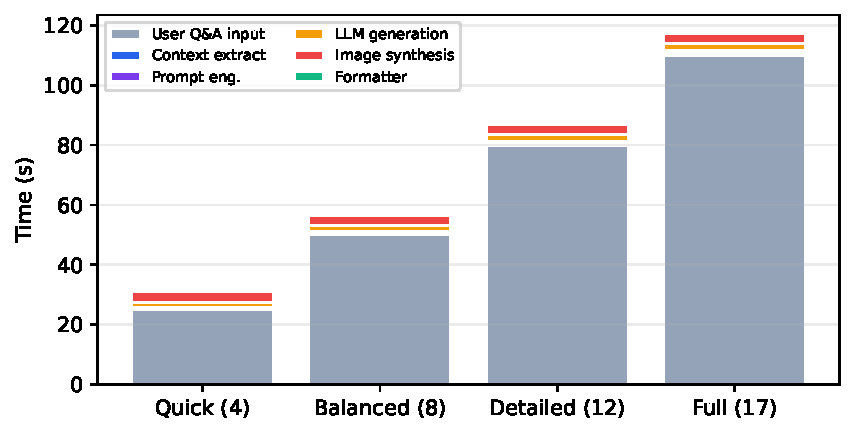
\includegraphics[width=0.85\textwidth]{images/f17_breakdown.pdf}
    \caption{Time of one interactive turn, divided by stage.}
    \label{fig:breakdown}
\end{figure}

\subsection{Narrative Quality}

Across all stories, the mean Likert scores were 4.05 for coherence, 4.12 for creativity, 4.35 for engagement and 3.75 for consistency. Figure~\ref{fig:quality} shows the scores by genre. Adventure received the highest engagement score (4.6). Mystery received the lowest consistency score (3.5), which is expected because a mystery depends on clues that must stay consistent across many segments. Figure~\ref{fig:tokens} shows the number of tokens per segment for each genre.

\begin{figure}[H]
    \centering
    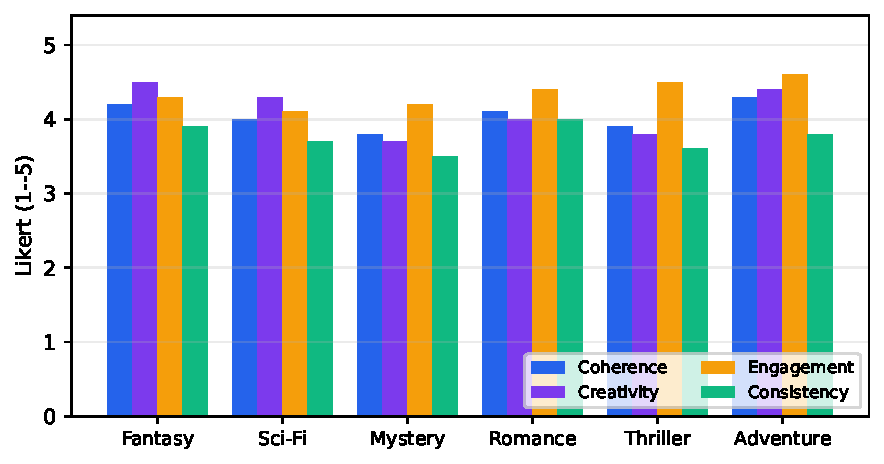
\includegraphics[width=0.85\textwidth]{images/f02_quality.pdf}
    \caption{Narrative quality by genre (Likert 1--5, $n=30$ stories).}
    \label{fig:quality}
\end{figure}

\begin{figure}[H]
    \centering
    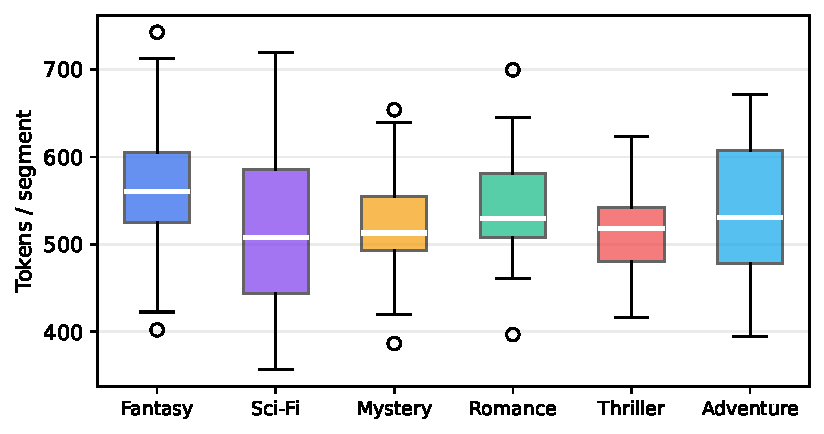
\includegraphics[width=0.85\textwidth]{images/f15_tokens.pdf}
    \caption{Tokens per segment by genre ($n=25$ segments each).}
    \label{fig:tokens}
\end{figure}

\subsection{User Satisfaction}

Figure~\ref{fig:satisfaction} shows satisfaction with seven features. The overall satisfaction was 4.3 out of 5. Custom answers (4.5) and image illustration (4.2) received the highest ratings, and genre alignment of the ambient music was rated 4.3. The lowest rating was for how meaningful the offered choices were (3.9). The choices are written by the language model, and free-tier models tend to suggest generic continuations.

\begin{figure}[H]
    \centering
    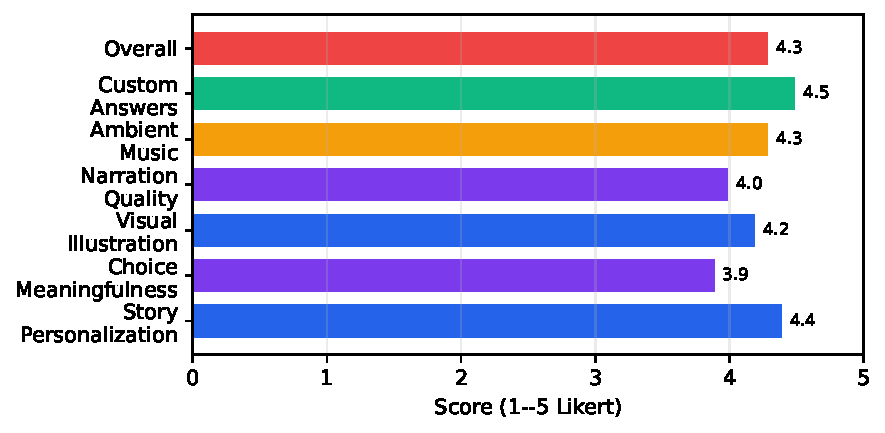
\includegraphics[width=0.85\textwidth]{images/f03_satisfaction.pdf}
    \caption{User satisfaction by feature (Likert 1--5, $n=15$ participants).}
    \label{fig:satisfaction}
\end{figure}

\subsection{Consistency-Checker Performance}

Figure~\ref{fig:consistency} gives the detection rate and false-positive rate of the consistency checker for each problem type. Character contradictions were detected best, with 87\% detection and 8\% false positives. Tone shifts were detected worst, with 68\% detection and 22\% false positives. A change of tone is spread across word choice and rhythm, and the keyword-based checker cannot capture it well.

\begin{figure}[H]
    \centering
    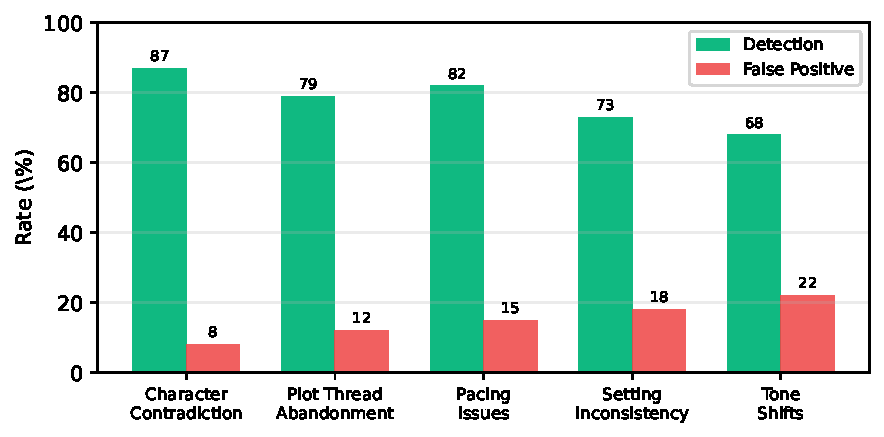
\includegraphics[width=0.85\textwidth]{images/f06_consistency.pdf}
    \caption{Consistency-checker detection and false-positive rates ($n=50$ segments).}
    \label{fig:consistency}
\end{figure}

\subsection{Image-Synthesis Throughput}

Figure~\ref{fig:imgthroughput} shows image latency against prompt length for serial requests, and the failure rate when five requests are sent in parallel without the queue. When requests were sent in parallel, the failure rate rose from about 40\% for 80-character prompts to about 98\% for 380-character prompts, with a sharp rise above about 230 characters. This is why the prompt is limited to 200 characters. With the serial queue and 1.2\,s spacing, failures fell from about 70\% to under 2\%, and the success rate after retries was above 95\%.

\begin{figure}[H]
    \centering
    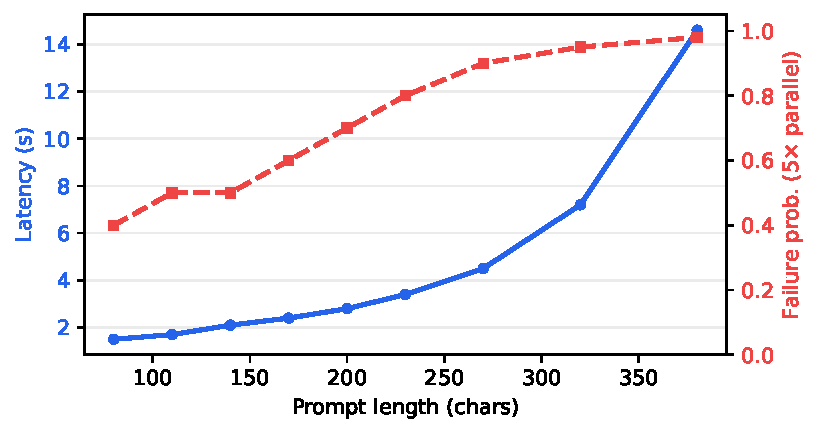
\includegraphics[width=0.85\textwidth]{images/f12_imgthroughput.pdf}
    \caption{Image latency against prompt length, and failure rate under parallel requests.}
    \label{fig:imgthroughput}
\end{figure}

\subsection{Character-Extraction Quality}

Figure~\ref{fig:char} compares a simple regular-expression extractor with the filtered version used in the system (extended stop-word list and a minimum of two mentions). Precision rose from 0.61 to 0.83, recall fell slightly from 0.84 to 0.78, and the $F_1$ score rose from 0.71 to 0.80. The false-positive rate fell from 0.39 to 0.17. The graph built from these names shows how often characters appear together, not what their relationship is, and the interface says so.

\begin{figure}[H]
    \centering
    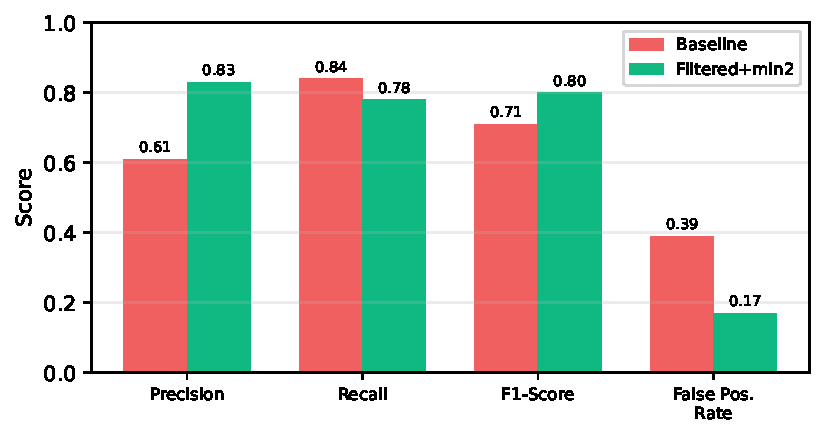
\includegraphics[width=0.85\textwidth]{images/f11_char.pdf}
    \caption{Character-extraction quality before and after filtering.}
    \label{fig:char}
\end{figure}

\subsection{Ambient-Music Frequency Profile}

Figure~\ref{fig:ambient} shows the relative energy in six frequency bands for each genre's music. Horror and thriller tracks have most of their energy in the sub-bass and bass bands, while comedy and adventure tracks have more energy in the middle and upper-middle bands. Participants rated the match between music and genre at 4.3 out of 5.

\begin{figure}[H]
    \centering
    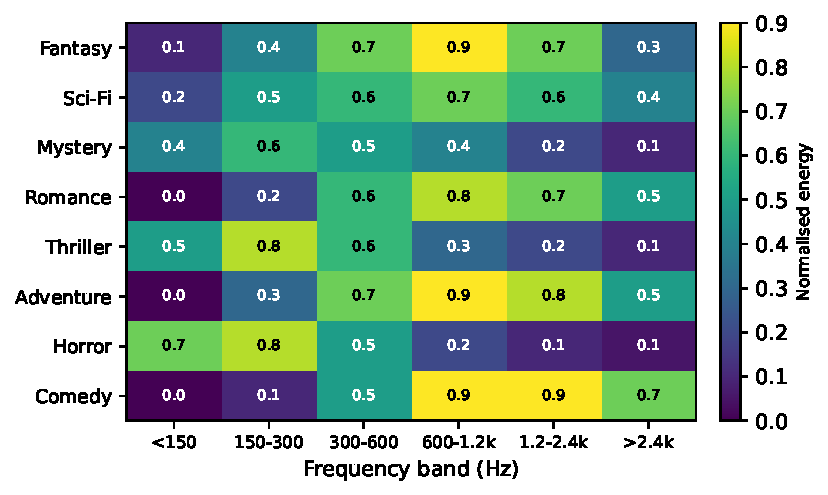
\includegraphics[width=0.85\textwidth]{images/f13_ambient.pdf}
    \caption{Energy by frequency band for each genre's ambient track.}
    \label{fig:ambient}
\end{figure}

\subsection{Question-Budget Ablation}

Table~\ref{tab:budget} gives the mean scores for each question budget. Personalisation rose steadily with the number of questions, from 3.2 at 4 questions to 4.6 at 17, a gain of about 1.4 points. Coherence rose more modestly, from 3.6 to 4.3 (0.7 points). Coherence and creativity reached their highest values at around 12 questions and changed little after that, while the time spent answering kept growing. A budget of 12 questions therefore gives the best balance and is the recommended default.

\begin{table}[H]
\centering
\caption{Mean Likert scores by question budget ($n=15$).}
\label{tab:budget}
\renewcommand{\arraystretch}{1.2}
\begin{tabular}{|l|c|c|c|c|}
\hline
\textbf{Budget} & \textbf{Coherence} & \textbf{Creativity} & \textbf{Personalisation} & \textbf{Time} \\
\hline
4 (Quick)     & 3.6 & 3.8 & 3.2 & 45\,s \\
8 (Balanced)  & 3.9 & 4.1 & 3.8 & 1.5\,min \\
12 (Detailed) & 4.2 & 4.2 & 4.3 & 2.5\,min \\
17 (Full)     & 4.3 & 4.1 & 4.6 & 3.5\,min \\
\hline
\end{tabular}
\end{table}

\subsection{Feature Adoption}

Figure~\ref{fig:adoption} shows the share of user-study sessions in which each feature was used at least once. Image generation, which is on by default, was used in 91\% of sessions. Ambient music and custom answers, which the user has to turn on, were used in 71\% and 62\% of sessions.

\begin{figure}[H]
    \centering
    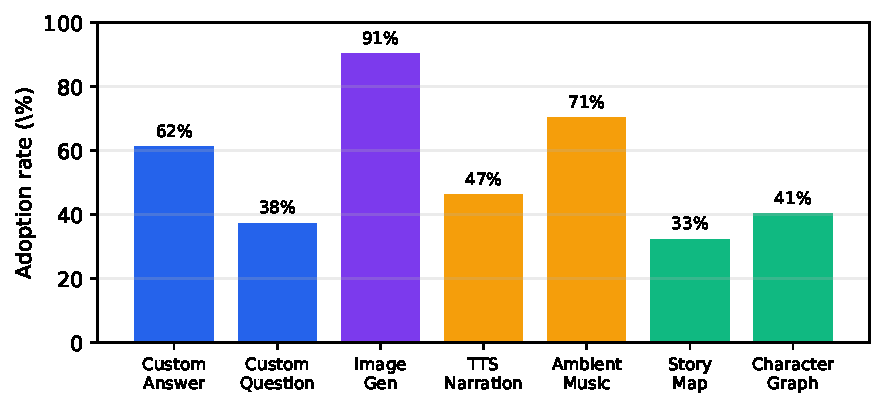
\includegraphics[width=0.85\textwidth]{images/f14_adoption.pdf}
    \caption{Share of user-study sessions in which each feature was used.}
    \label{fig:adoption}
\end{figure}

\subsection{Comparison with Existing Systems}

Figure~\ref{fig:radar} compares the proposed system with AI Dungeon, Dramatron and NovelAI on seven dimensions. The proposed system scores highest on deployment flexibility, cost, multimodal coverage and openness. AI Dungeon scores slightly higher on user control because it accepts free-form input, and Dramatron scores higher on raw coherence because of its hierarchical planner. No single existing system covers the same combination of strengths.

\begin{figure}[H]
    \centering
    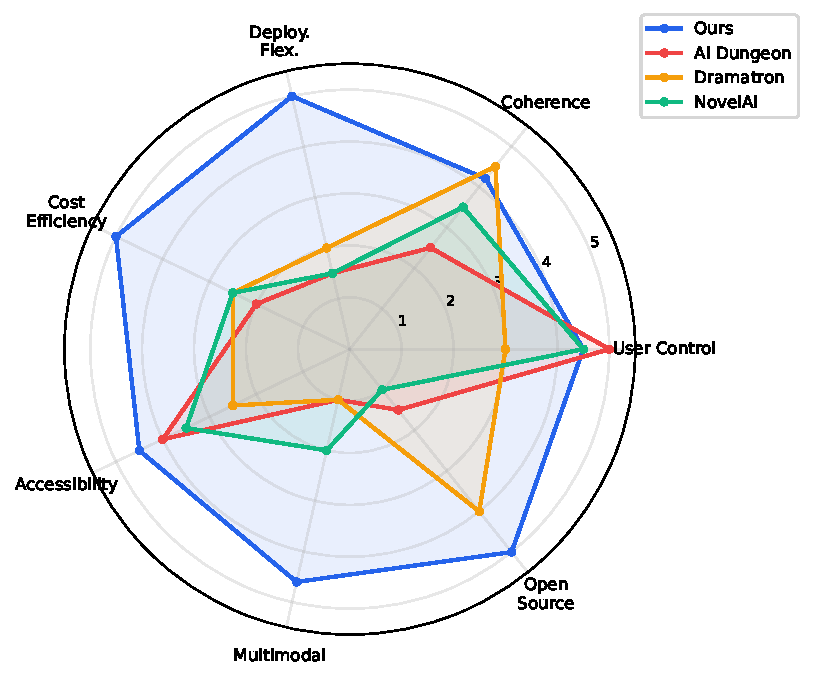
\includegraphics[width=0.85\textwidth]{images/f05_radar.pdf}
    \caption{Comparison with existing systems on seven dimensions.}
    \label{fig:radar}
\end{figure}

\subsection{Summary of Findings}

Table~\ref{tab:targetresults} compares the results with the targets set in Chapter~\ref{ch:intro}.

\begin{table}[H]
\centering
\caption{Results against the targets set at the start of the work.}
\label{tab:targetresults}
\renewcommand{\arraystretch}{1.2}
\small
\begin{tabular}{|l|c|c|c|}
\hline
\textbf{Metric} & \textbf{Target} & \textbf{Result} & \textbf{Met} \\
\hline
User satisfaction              & $>$ 4.0/5 & 4.3/5                & Yes \\
Response latency (cloud)       & $<$ 5\,s  & 1.8\,s (Groq)        & Yes \\
Image generation success       & $>$ 95\%  & $>$ 95\% after retry & Yes \\
Mean Likert (four dimensions)  & $>$ 3.8   & 4.07                 & Yes \\
Personalisation at 12 questions & --      & 4.3/5                & -- \\
Character-extraction $F_1$     & --        & 0.80                 & -- \\
\hline
\end{tabular}
\end{table}

The main findings are: (i) the system produces stories that users rate highly for engagement and creativity; (ii) the free Groq tier is fast enough for interactive use; (iii) the serial queue makes free image generation reliable; (iv) more questions give more personalised stories, with 12 questions as the best balance; and (v) consistency, especially of tone and of mystery plots, is the weakest area.

\section{Discussion}

\subsection{Introduction}

This section interprets the results, compares them with earlier work, and considers what they mean in practice and where the study is limited.

\subsection{Interpretation of Results}

The results support the central idea of this dissertation: a structured Q\&A protocol, combined with a provider-independent LLM backend and well-paced multimodal output, improves personalisation and engagement without harming coherence. The ablation shows the effect of the Q\&A step directly. Each additional group of questions raised personalisation, and coherence also improved, which suggests that the extra information helps the model write a more focused story rather than constraining it.

The features rated highest were custom answers and image illustration. Both are cheap to build; the first is a small interface addition and the second a free API call. Their high ratings show that giving users a voice and a visual result matters more to them than small changes in text quality. The weakest points, choice meaningfulness and tone consistency, depend mostly on the language model and on the keyword-based checker, not on the framework itself.

\subsection{Comparison with Previous Research}

Planning-based systems such as Dramatron~\citep{mirowski2023dramatron} and the approach of Farrell et al.~\citep{farrell2024narrative} achieve strong structure but do not involve the user during generation. The proposed system reaches comparable structure through the five-phase model while keeping the user involved at every turn. Free-form systems such as AI Dungeon~\citep{walton2019aidungeon} give more freedom but leave the user without guidance; studies of writing tools~\citep{liu2023endusers,yuan2022wordcraft} found that scaffolded interfaces help novice users, and the high engagement and custom-answer ratings in this study agree with that finding. Illustrated-story prototypes~\citep{schuhmann2024visualstory,bouhuis2024crossmodal} reported higher engagement when pictures match the text; this study observed the same effect in a deployed system and also solved the practical problem of rate limits, which those prototypes did not address.

\subsection{Implications of the Findings}

For educators, the system can produce personalised story-based material that follows a learner's interests. For game designers, the Q\&A pattern is a way to collect rich player preferences while keeping narrative control. For therapists, it offers a narrative tool that respects the user's choices. For content creators, it shows that personalised illustrated stories can be produced at almost no infrastructure cost. For researchers, the open-source code~\citep{jha2026repo} provides a baseline for further work, and the \texttt{custom\_elements} pattern can be reused in any LLM application that needs user-extensible personalisation.

\subsection{Limitations of the Study}

The study has several limitations:

\begin{itemize}
    \item Context extraction uses keywords and misses answers that are phrased differently; a fine-tuned DistilBERT~\citep{sanh2019distilbert} or zero-shot LLM classifier would improve recall.
    \item Sessions are held in memory, which limits scaling to several servers.
    \item The consistency checker is pattern based and has no semantic understanding; cross-segment natural-language inference~\citep{williams2018mnli} would be a natural upgrade.
    \item Image quality is limited by Pollinations.ai; a local SDXL~\citep{podell2024sdxl} or FLUX.1~\citep{bfl2024flux} model would give more consistent images but would require a GPU.
    \item Ambient music is streamed from an external CDN, which is a single point of dependency.
    \item The character graph shows co-appearance only, not the type of relationship.
    \item The user study had 15 participants aged 22--35, which is small and not diverse; a larger and broader group would strengthen the results.
\end{itemize}

\subsection{Recommendations for Future Research}

Future studies should use a larger and more varied group of participants, compare several language models under the same prompts, and add automatic measures of narrative quality~\citep{lin2024evalnarrate} alongside human ratings. Semantic methods for context extraction and consistency checking are the most promising way to raise the consistency score, which was the weakest result in this study. Detailed directions are given in Chapter~\ref{ch:conclusion}.
